\documentclass[11pt,a4paper]{article}
\usepackage[T1]{fontenc}
\usepackage[utf8]{inputenc}
\usepackage{lmodern,microtype}
\usepackage{amsmath,amssymb,amsthm,mathtools,bm}
\usepackage{booktabs,array,tabularx,longtable}
\usepackage{graphicx,float,caption}
\usepackage{xcolor}
\usepackage[margin=20mm]{geometry}
\usepackage{enumitem,fancyhdr}
\usepackage[hidelinks,unicode=true]{hyperref}
\hypersetup{
 pdftitle={FIN ST154--ST165: Interaction-Generated Algebras, Minimal Anisotropy, and Operational Completion},
 pdfauthor={Krzysztof Żuchowski},
 pdfsubject={Analytical and computational execution of FIN programs ST154--ST165},
 pdfkeywords={FIN, superselection, operator algebra, Krawczyk, quantum recovery, symmetry breaking, anisotropy, hidden Markov model, thermal operation, spectrahedron, operational theory}
}
\setlength{\parindent}{0pt}
\setlength{\parskip}{0.48em}
\setlength{\emergencystretch}{2em}
\setlength{\headheight}{14pt}
\setlist[itemize]{leftmargin=1.55em,itemsep=0.14em,topsep=0.2em}
\setlist[enumerate]{leftmargin=1.75em,itemsep=0.14em,topsep=0.2em}
\pagestyle{fancy}\fancyhf{}
\lhead{FIN ST154--ST165}\rhead{Release 10.67}\cfoot{\thepage}
\newtheorem{theorem}{Theorem}[section]
\newtheorem{proposition}[theorem]{Proposition}
\newtheorem{corollary}[theorem]{Corollary}
\newcommand{\proven}{\textcolor{green!40!black}{\textbf{[PROVEN]}}}
\newcommand{\strong}{\textcolor{blue!70!black}{\textbf{[STRONG EVIDENCE]}}}
\newcommand{\conditional}{\textcolor{violet!65!black}{\textbf{[CONDITIONAL]}}}
\newcommand{\openstatus}{\textcolor{red!72!black}{\textbf{[OPEN]}}}
\newcommand{\statusboundary}{\textcolor{orange!80!black}{\textbf{[BOUNDARY]}}}
\newcommand{\resultbox}[1]{\begin{center}\fcolorbox{blue!60!black}{blue!4}{\parbox{0.92\textwidth}{#1}}\end{center}}

\begin{document}
\pagenumbering{gobble}
\begin{titlepage}
\centering
\vspace*{0.85cm}
{\LARGE\bfseries FIN ST154--ST165\par}
\vspace{0.28cm}
{\Large Interaction-Generated Algebras, Minimal Anisotropy, and Operational Completion\par}
\vspace{0.40cm}
{\large Environment-induced fixed algebras, enlarged fold certificates, orthogonal-unitary recovery, sharp preparation action, the first local $C_{12}$ anisotropy, adaptive nuisance covers, functorial refinement, instrument-tomographic causal nets, hidden-HMM inference, finite-time bath bounds, minimax extreme geometry, and an axiom-deleted operational FIN tuple\par}
\vspace{0.75cm}
{\Large Krzysztof \.{Z}uchowski\par}
\vspace{0.18cm}
{\large Independent Researcher --- Fractal Information Theory Project\par}
{\large ORCID: 0009-0002-0909-3613\par}
\vspace{0.55cm}
{\large FIN Release 10.67 --- Version 1.0.0\par}
{\large August 11, 2026\par}
\vfill
\begin{minipage}{0.92\textwidth}
\textbf{Research question.} Can the missing observable algebra, selector dynamics, carrier-independent information, and thermal resources be derived without inserting their operational meaning by hand?\par
\textbf{Methods.} Finite fixed-point algebras, commutant computation, outward interval Krawczyk proof, quantum-channel recovery, sharp variational inequalities, cyclic invariant theory, affine cohomology, instrument tomography, hidden-Markov transfer bounds, diamond-norm speed limits, spectrahedral geometry, and typed axiom deletion.\par
\textbf{Epistemic rule.} The interaction, preparation metric, nonlinear coupling, tomography table, bath, clock, and record remain supplied whenever they are not strict-derived. A numerical cluster is never promoted to a theorem.\par
\textbf{Repository snapshot.} Audited tracked base commit \texttt{8a4c9b0b29b4fed8f7dcdc86e79b98306818efea}. The working tree contains earlier local research artifacts; this release has its own SHA-256 manifest.\par
\textbf{Repository.} \url{https://github.com/hyconiek/Fractal-Nadsoliton-Theory}\par
\textbf{License.} CC BY 4.0.
\end{minipage}
\end{titlepage}
\pagenumbering{arabic}

\begin{abstract}
ST154--ST165 execute the next local, falsification-first FIN research batch. ST154 proves that a finite-dimensional dephasing environment selects the joint commutant of its Hamiltonian and interaction observables. This constructs an observable algebra without naming it as output, but not without typing the interaction. Monitoring the strict operator $A$ leaves its $22$-dimensional commutant; monitoring a supplied nondegenerate vertex observable leaves a $12$-dimensional diagonal algebra; monitoring both leaves only scalars. None produces the desired fine-blind algebra from strict data alone.

ST155 adaptively retests all 35 numerical fold clusters. Thirty-one now have interval Krawczyk certificates and larger uniqueness boxes, up from 29. The remaining four are not certified, and the union of local neighborhoods is not a global domain cover. ST156 proves optimal recovery for arbitrary finite Hilbert--Schmidt-orthogonal unitary error families with classical noisy syndrome. ST157 proves the sharp finite-time preparation action $11g^2/(24T)$ for a declared probability-simplex metric.

ST158 obtains a new exact structural result. On the normalized first Fourier mode of $C_{12}$, every local even monomial below degree twelve is angularly isotropic. Degree twelve is the first that produces anisotropy, through
\[
\sum_{j=0}^{11}\cos^{12}(\theta+2\pi j/12)=\frac{693}{256}+\frac{3}{512}\cos(12\theta).
\]
Thus the lattice fixes the first allowed anisotropy shape and its projection factor, but not the nonlinear coupling, sign, units, or source. ST159 partitions a nuisance cube of halfwidth $5\times10^{-5}$ into 64 interval cells and proves inclusion in every cell. The previous single-box failure at $1.46\times10^{-5}$ was a proof-method boundary, not root loss.

ST160 proves functorial coarse-graining for all-odd refinement cohomology. ST161 gives a noiseless instrument-tomography criterion for recovering a labeled atomic causal net. ST162 corrects and certifies finite-count discrimination in a fully hidden non-erasure HMM, including a positive conservative exponent. ST163 combines the bath-dimension lower bound with a general bounded-generator speed limit and a two-site SWAP upper construction. ST164 proves that the minimax optimizer spectrahedron has affine dimension $66$, gives a complete linear extremality criterion, and certifies at least $4{,}213{,}597$ partition extreme points. ST165 packages eleven independently typed operational atoms and supplies deletion witnesses. No strict environment coupling, selector, dimensional scale, apparatus, physical projection, or Theory-of-Everything closure follows.
\end{abstract}

\textbf{Status vocabulary.} \proven{} means exact analytic, finite, or source-code interval proof in the displayed scope. \conditional{} means explicit extra resources are used. \strong{} marks numerical evidence only. \openstatus{} is an unclosed goal. \statusboundary{} records a non-implication.

\tableofcontents
\newpage

\section{Frozen core and kernel discipline}

The strict working operator remains
\begin{equation}
W_{xx}=0,\qquad
W_{xy}=\frac{\cos(0.18575d(x,y)+0.16250)}{1+d(x,y)^{9/5}}\quad(x\ne y),
\qquad A=sI-W,
\label{eq:strict}
\end{equation}
on $C_{12}$, with $s=2\sum_{d=1}^{5}W(d)+W(6)$. Hence
\[
\langle f,Af\rangle=\frac12\sum_{x,y}W_{xy}|f_x-f_y|^2\ge0.
\]
The legacy ontological kernel remains an intermediate bridge kernel. This release neither identifies it with~\eqref{eq:strict} nor transfers proposed legacy electroweak, electromagnetic, or hierarchy roles. The nadsoliton remains the primordial fractal information in solitonic state, not an object above a deeper information layer.

\resultbox{\textbf{Central result.} The missing algebra can be generated by an environment only after its interaction observable is specified. The missing $C_{12}$ anisotropy shape can be generated by local degree-twelve nonlinearity, but its coupling remains unspecified. These are genuine structural advances, yet both locate the remaining physical source outside strict functional calculus.}

\section{Outcome matrix}
\small
\begin{longtable}{@{}p{0.06\textwidth}p{0.25\textwidth}p{0.31\textwidth}p{0.31\textwidth}@{}}
\toprule ID & Target & Result & Boundary\\\midrule\endfirsthead
\toprule ID & Target & Result & Boundary\\\midrule\endhead
ST154 & Environment-induced algebra & \proven{} fixed algebra equals joint commutant & Interaction and dephasing law supplied\\
ST155 & Fold neighborhood cover & \proven{} 31 certified roots and exclusion shells & Not a full 15D domain cover\\
ST156 & General coherent recovery & \proven{} for finite orthogonal unitary families & Nonorthogonal errors open\\
ST157 & Physical selector cost proxy & \conditional{} sharp kinetic action bound & Metric, clock, gap, and outcome supplied\\
ST158 & Source shape of anisotropy & \proven{} degree 12 is minimal; exact coefficient & Coupling $g$ and sign remain missing\\
ST159 & Nuisance continuation & \proven{} all 64 cells pass at global $h=5\times10^{-5}$ & Maximal domain not located\\
ST160 & Refinement functor & \proven{} all-odd coboundary and coarse-graining theorem & Refinement graph supplied\\
ST161 & Causal-net recovery & \proven{} exact noiseless tomography criterion & Noise and physical labels open\\
ST162 & Fully hidden counts & \proven{} exact finite errors and positive upper-error exponent & Model and emissions supplied\\
ST163 & Local bath/time cost & \proven{} speed lower bound and site-local SWAP construction & Microscopic locality and units open\\
ST164 & Minimax extreme geometry & \proven{} dimension and complete linear criterion & Full extreme list not enumerated\\
ST165 & Operational completion & \conditional{} eleven-atom deletion map & No laboratory instantiation or independent custody\\
\bottomrule
\end{longtable}
\normalsize

\section{ST154: interaction-generated superselection algebras}

For Hermitian interaction observables $L_k$, consider the Heisenberg generator
\[
\mathcal L^*(X)=i[H,X]-\frac12\sum_k[L_k,[L_k,X]].
\]
Taking the Hilbert--Schmidt inner product with $X$ shows that a fixed point must commute with every $L_k$; the Hamiltonian part separately requires commutation with $H$.

\begin{theorem}[Finite dephasing fixed algebra]
The fixed observable algebra is
\[
\operatorname{Fix}(e^{t\mathcal L^*})=\{H,L_1,\ldots,L_m\}'.
\]
Thus an environment may generate its pointer algebra as output, but the interaction observables remain typed input.
\end{theorem}

For the strict system the computed complex dimensions are
\[
\dim\{A\}'=22,\qquad \dim\{Q_{\rm vertex}\}'=12,
\qquad \dim\{A,Q_{\rm vertex}\}'=1,
\]
while $A\otimes I_2$ has commutant dimension $88$. The joint scalar result follows because $Q_{\rm vertex}=\operatorname{diag}(0,\ldots,11)$ has simple spectrum and the connected strict graph couples every vertex.

\begin{figure}[H]\centering
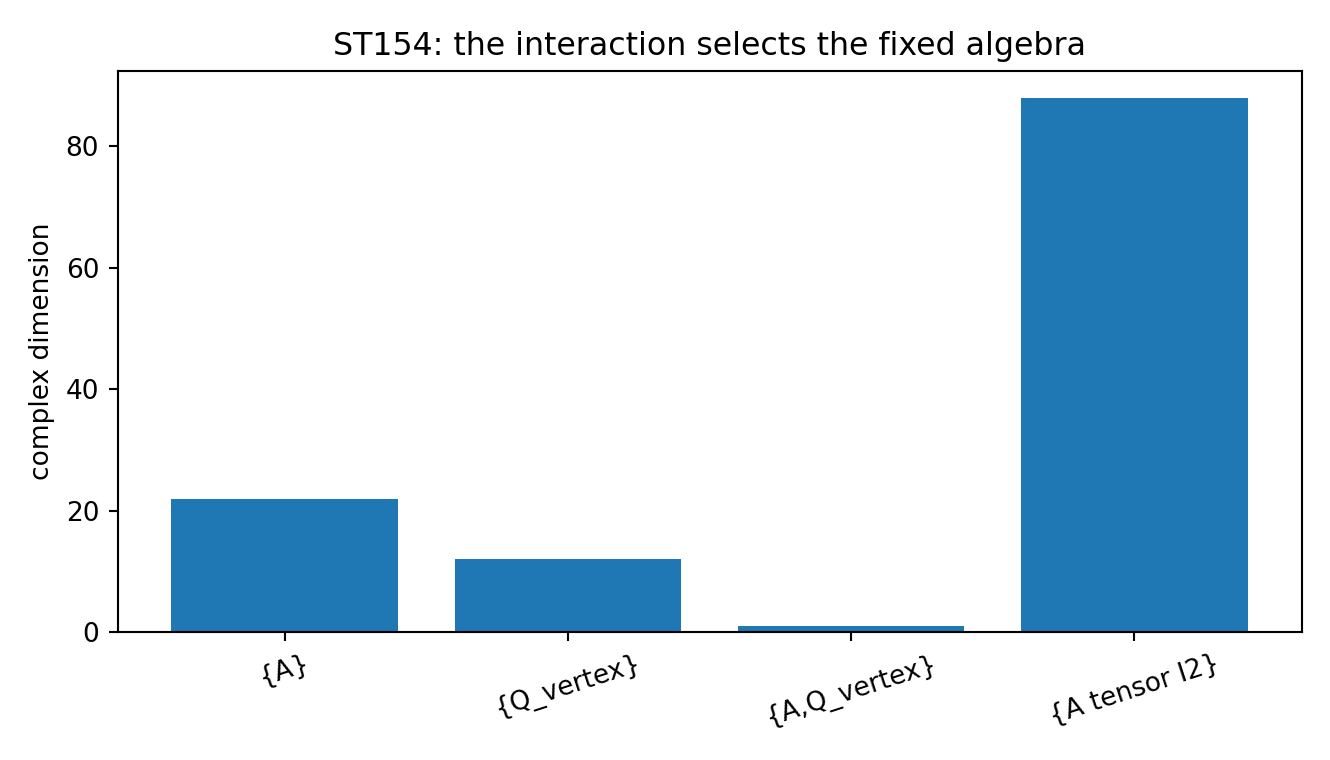
\includegraphics[width=.76\textwidth]{FIN_ST154_ST165_Figures/st154_fixed_algebras.png}
\caption{ST154. Different supplied interactions generate different fixed algebras. Strict monitoring alone preserves the 22-dimensional spectral commutant.}
\end{figure}

The result answers the superselection question precisely: the algebra can emerge from a coupling without being named in advance, but the coupling cannot be omitted. Neither strict $A$ nor full naturality chooses the desired fine-blind algebra.

\section{ST155: enlarged fold certificates without false completeness}

All 35 representatives from ST144 were retested at radii
\[
10^{-4},3\cdot10^{-5},10^{-5},\ldots,10^{-10}.
\]
Each accepted Krawczyk box proves exactly one root in that box. Thirty-one representatives now pass, including two clusters previously outside the certificate budget. Twenty-eight accept a tested radius $10^{-4}$ and three accept $10^{-5}$. Four clusters near the small-amplitude and $\kappa\approx-0.0695$ regions remain uncertified.

\begin{theorem}[Local union and exclusion shells]
At least 31 distinct local fold roots exist. For every certified center, both the radius-$10^{-7}$ box and a strictly larger box pass. Hence the max-norm shell between them contains no additional root.
\end{theorem}

\begin{figure}[H]\centering
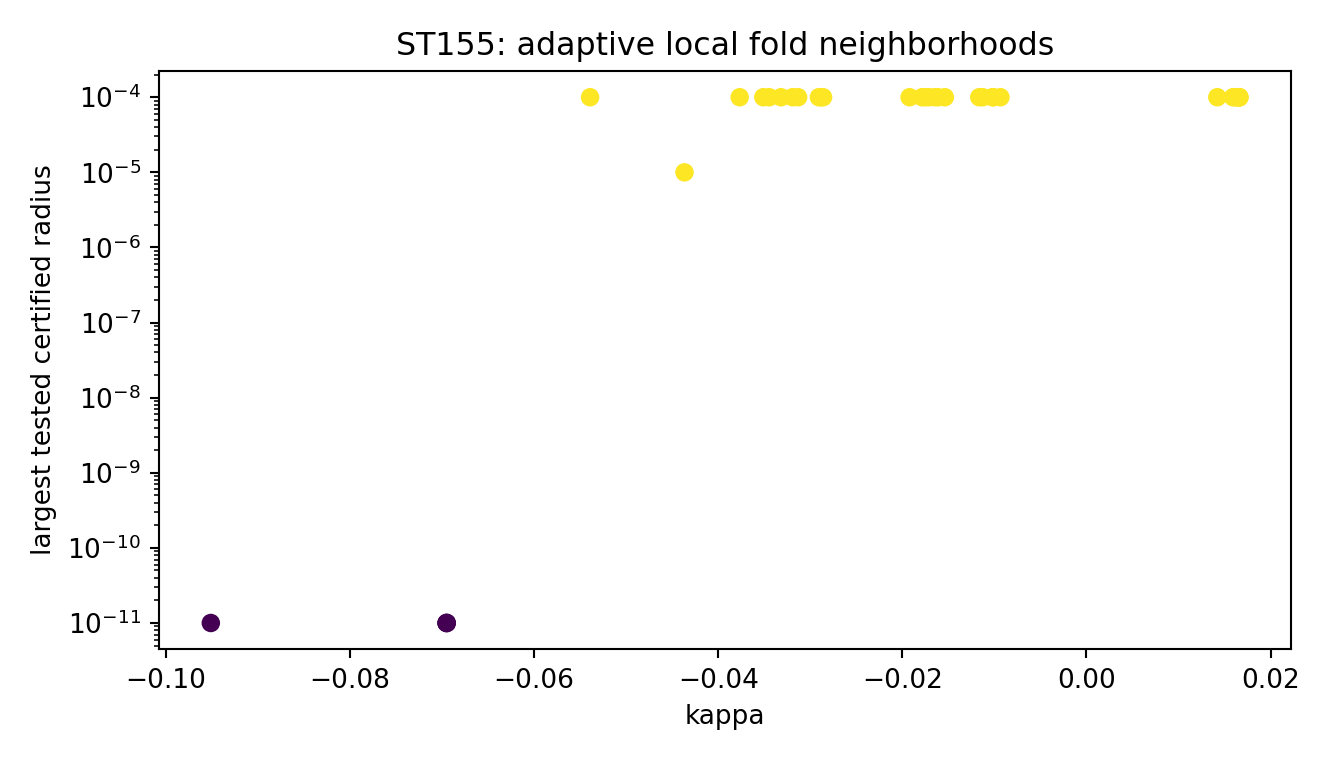
\includegraphics[width=.76\textwidth]{FIN_ST154_ST165_Figures/st155_fold_neighborhoods.png}
\caption{ST155. Largest tested accepted radius for each numerical cluster; four representatives remain uncertified.}
\end{figure}

\statusboundary{} Thirty-one is a proved lower bound, not the exact global root count. The local boxes do not cover the filtered 15-dimensional domain, so roots outside them remain possible.

\section{ST156 and ST157: recovery and preparation-resource cost}

\subsection{Orthogonal-unitary leakage with noisy syndrome}

Let $\{U_a\}$ be Hilbert--Schmidt-orthogonal unitaries,
\[
\operatorname{Tr}(U_a^\dagger U_b)=d\delta_{ab},
\]
with prior $p_a$ and classical readout channel $q(y|a)$. Conditional on syndrome $y$, applying $U_a^\dagger$ for the maximum-posterior label is optimal.

\begin{theorem}[Orthogonal-unitary recovery]
For every finite orthogonal unitary error family,
\[
F_e^*=\sum_y\max_a p_aq(y|a).
\]
\end{theorem}

Parseval's identity for the matrix Hilbert space bounds every CPTP recovery by the largest conditional error weight; inverse-unitary correction attains it. The four-error $12$-dimensional example has prior $(0.55,0.25,0.15,0.05)$, asymmetric cyclic readout, and
\[
F_e^*=0.78,
\]
compared with $0.55$ when syndrome data are ignored.

\begin{figure}[H]\centering
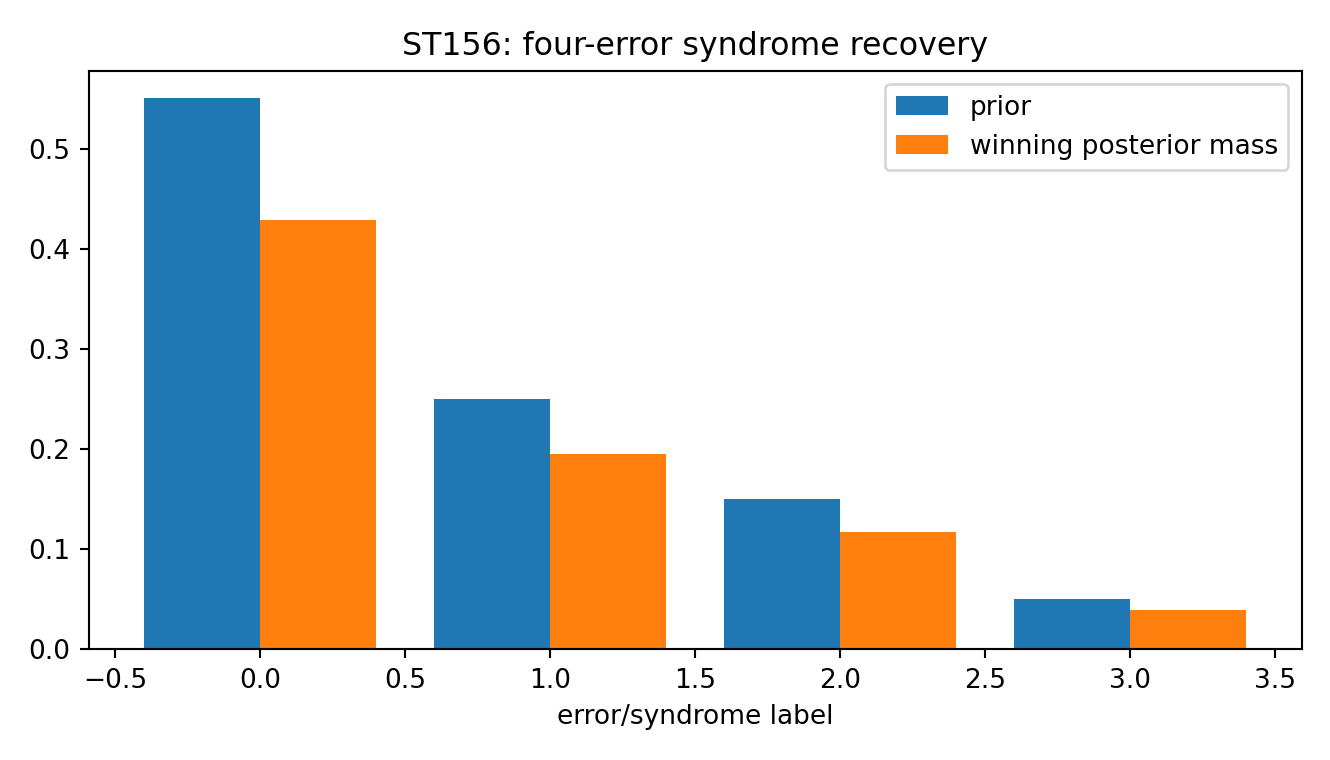
\includegraphics[width=.73\textwidth]{FIN_ST154_ST165_Figures/st156_unitary_recovery.png}
\caption{ST156. Error prior and winning posterior mass for each reported syndrome.}
\end{figure}

\subsection{A sharp kinetic preparation bound}

Let $p(0)=u=(1/12,\ldots,1/12)$ and demand $p_0(T)-p_j(T)\ge g$. For the declared kinetic action
\[
\mathcal A[p]=\frac12\int_0^T\|\dot p(t)\|_2^2\,dt,
\]
Cauchy--Schwarz and the least-asymmetric endpoint give
\begin{equation}
\mathcal A[p]\ge\frac{\|p(T)-u\|_2^2}{2T}
=\frac{11g^2}{24T}.
\label{eq:action}
\end{equation}
The straight probability path attains equality. If instantaneous kinetic power is bounded by $P_{\max}$, then
\[
T\ge\frac{\sqrt{11/12}\,g}{\sqrt{2P_{\max}}}.
\]

\begin{figure}[H]\centering
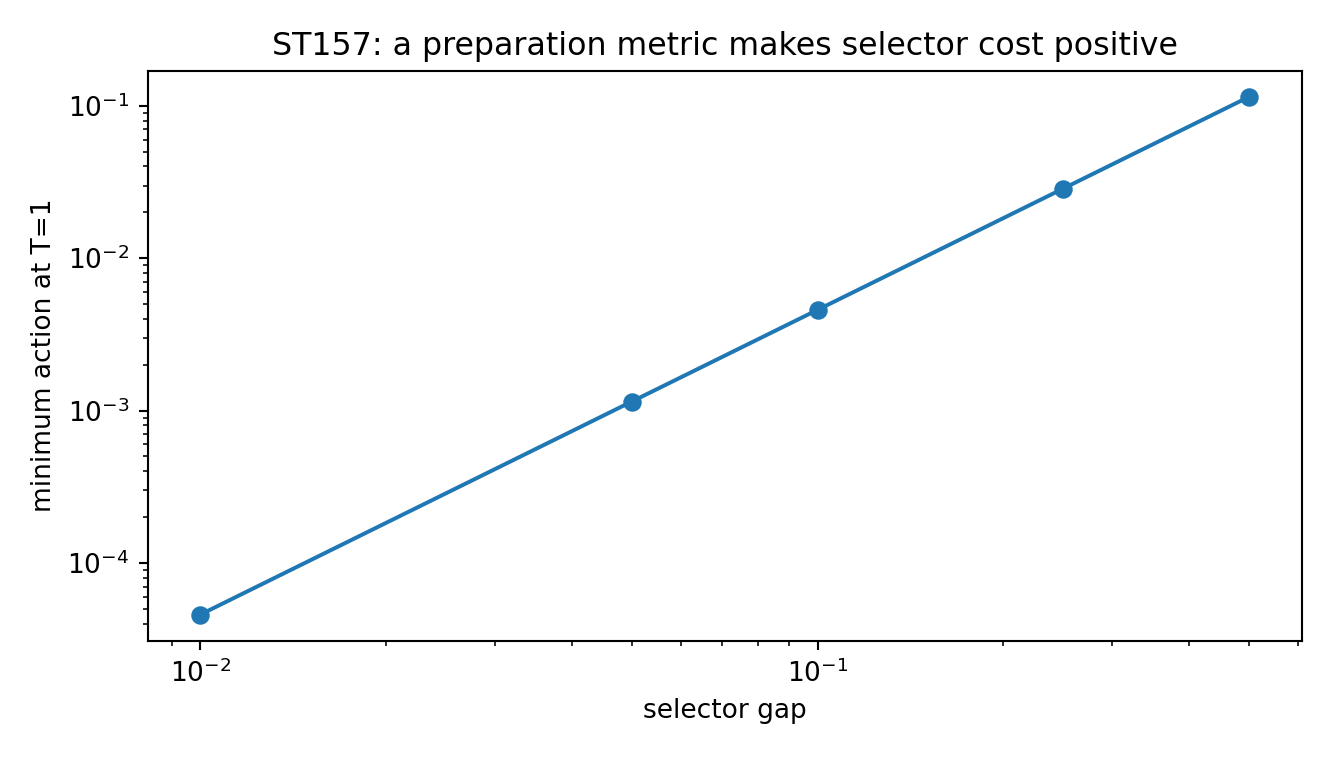
\includegraphics[width=.72\textwidth]{FIN_ST154_ST165_Figures/st157_action_cost.png}
\caption{ST157. Exact minimum quadratic preparation action for unit horizon.}
\end{figure}

\conditional{} Equation~\eqref{eq:action} makes selection costly only after choosing a Euclidean control metric, preferred outcome, gap, and time horizon. It is not a derivation of physical action, joules, or seconds from FIN.

\section{ST158: the first local \texorpdfstring{$C_{12}$}{C12} anisotropy}

On the normalized first real Fourier mode, write
\[
\psi_j=\frac r{\sqrt6}\cos\left(\theta+\frac{2\pi j}{12}\right).
\]
Discrete Fourier aliasing removes all angular harmonics of local even monomials below degree twelve. At degree twelve,
\begin{align}
\sum_{j=0}^{11}\cos^{12}\left(\theta+\frac{2\pi j}{12}\right)
&=\frac{693}{256}+\frac{3}{512}\cos(12\theta),\\
\sum_{j=0}^{11}\psi_j^{12}
&=\frac{r^{12}}{6^6}\left(\frac{693}{256}+\frac{3}{512}\cos(12\theta)\right).
\end{align}

\begin{theorem}[Minimal local anisotropy order]
Every local even vertex monomial $\sum_j\psi_j^{2m}$ with $2m<12$ is angularly constant on the first Fourier mode. Degree twelve is minimal and has the exact angular coefficient $3/(512\,6^6)$.
\end{theorem}

\begin{figure}[H]\centering
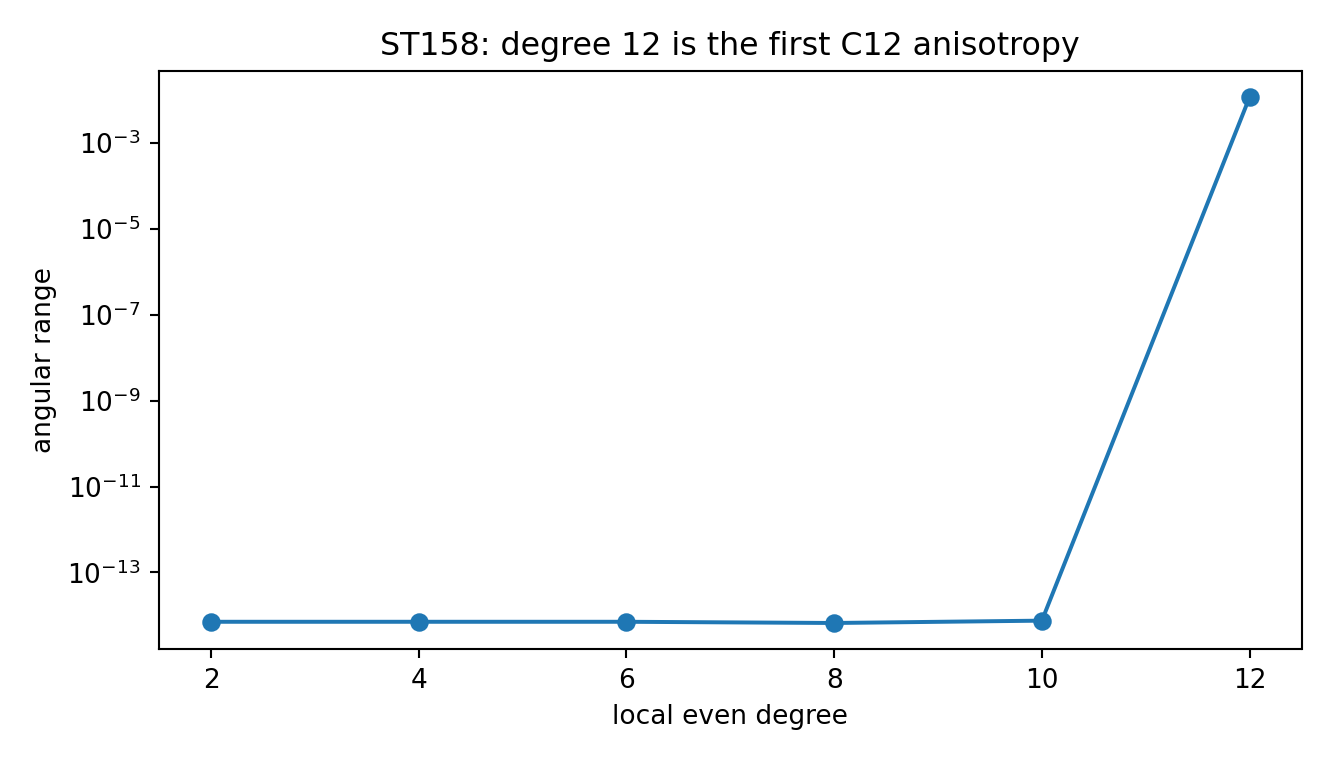
\includegraphics[width=.74\textwidth]{FIN_ST154_ST165_Figures/st158_anisotropy_order.png}
\caption{ST158. The angular range is zero up to numerical roundoff below degree twelve and becomes nonzero at degree twelve. The theorem itself is exact.}
\end{figure}

For the local interaction $(g/12)\sum_j\psi_j^{12}$, comparison with the ST147 convention gives
\[
\varepsilon=-\frac{3g}{512\,6^6}.
\]
This is the first strict-lattice mechanism producing the correct $\cos(12\theta)$ shape. It is not a strict source of $g$: the magnitude, sign, units, and physical origin of that coupling remain free.

\section{ST159: adaptive interval continuation}

The cube
\[
|q_0-0.2|\le5\times10^{-5},\quad
|q_1-0.7|\le5\times10^{-5},\quad
|\delta-0.05|\le5\times10^{-5}
\]
was partitioned into $4^3=64$ cells. Each cell uses its own numerical center, outward interval residual and Jacobian, and a local Krawczyk proof box.

\begin{theorem}[Uniform adaptive nuisance cover]
All 64 cells pass strict inclusion. Therefore every nuisance triple in the complete global cube possesses exactly one stationary root in its cell-specific certified root box. The smallest inclusion margin is
\[
1.345222066206242\times10^{-3}.
\]
\end{theorem}

\begin{figure}[H]\centering
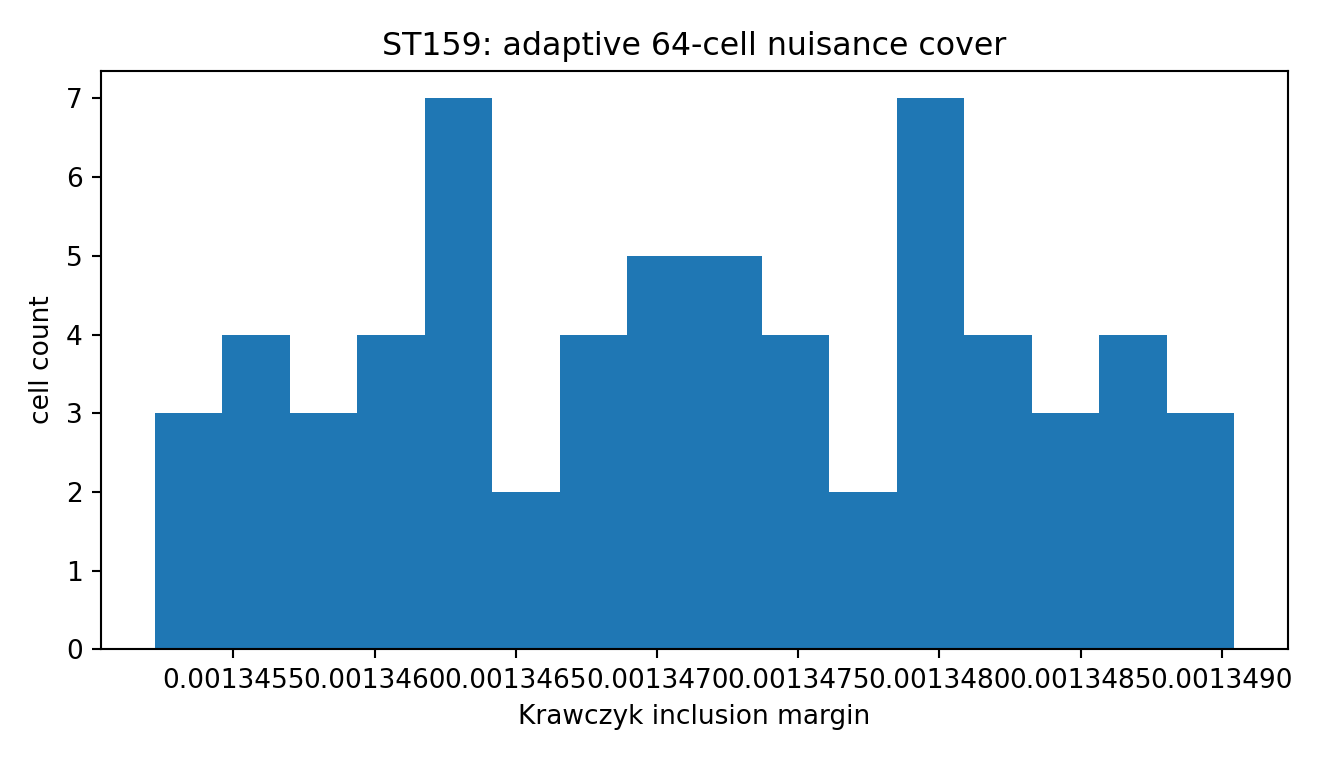
\includegraphics[width=.74\textwidth]{FIN_ST154_ST165_Figures/st159_adaptive_cover.png}
\caption{ST159. Distribution of the 64 positive Krawczyk margins.}
\end{figure}

The new global halfwidth exceeds the ST148 first single-box failure by more than a factor of three. That earlier threshold is therefore falsified as a geometric/root-loss boundary. The maximal continuation domain and global optimization remain open.

\section{ST160 and ST161: functorial refinement and causal-net recovery}

\subsection{Coarse-graining of all-odd twists}

For a rooted all-odd refinement DAG in which every vertex is reachable, a path-independent $\mathbb F_2$ edge twist is exactly a vertex coboundary
\[
b_{uv}=\phi_u+\phi_v.
\]
The coherent space therefore has dimension $|V|-1$. Retaining a subset of vertices pushes the twist forward by restricting $\phi$. The map is surjective and has kernel dimension equal to the number of eliminated nonroot vertices.

For the four-edge diamond, one coherence equation leaves eight assignments. Coarse-graining to one edge gives each coarse twist exactly four fine preimages. Mixed path parity remains an independent obstruction because affine linear parts must also agree.

\proven{} This makes the refinement certificate functorial in the declared all-odd category. \statusboundary{} The graph, parities, and twists remain supplied; no strict law of fractal refinement or compression is derived.

\subsection{Instrument tomography can reconstruct a typed net}

Exact tomography of labeled Pauli-complete left and right instrument families gives two commuting $M_2$ algebras, each of dimension four and each the commutant of the other. Their join has dimension sixteen and trivial commutant, hence equals $M_4$. Global unitary conjugation preserves this characterization. A single abelian $Z$ instrument instead generates dimension two and has commutant dimension eight.

\begin{theorem}[Noiseless atomic-net reconstruction]
Two labeled, commuting, tomographically reconstructed full $M_2$ factors that generate $M_4$ determine the two-factor net up to local unitaries. Labels remove the remaining swap ambiguity.
\end{theorem}

The theorem is operationally useful but conditional: completeness, exact matrices, labels, and their interpretation as physical regions are supplied.

\section{ST162: a genuinely hidden non-erasure HMM}

The availability state now remains hidden: every event is binary and neither symbol reveals the state. The common state transition is
\[
P=\begin{pmatrix}.9&.1\\.2&.8\end{pmatrix},\qquad
\pi=\left(\frac23,\frac13\right).
\]
The two hypotheses use hidden-state-dependent probabilities
\[
p_0=(0.02,0.08),\qquad p_1=(0.92,0.98).
\]

Exact forward enumeration gives Bayes error $0.05$ at one event, $2.1673\times10^{-4}$ at eight, and $8.1821\times10^{-8}$ at eighteen. The implementation initially omitted one first-event symbol; the test suite detected this, the enumeration was corrected, and all reported values were regenerated.

For $s=1/2$, subadditivity
\[
\left(\sum_i a_i\right)^s\le\sum_i a_i^s
\]
expands the observed Chernoff coefficient into a positive four-state pair-path transfer bound. Its spectral radius is $0.7211542215$, and every row sum is at most
\[
0.7939043352<1.
\]
Thus the conservative certified exponent is
\[
-\log(0.7939043352)=0.2307923097>0.
\]

\begin{figure}[H]\centering
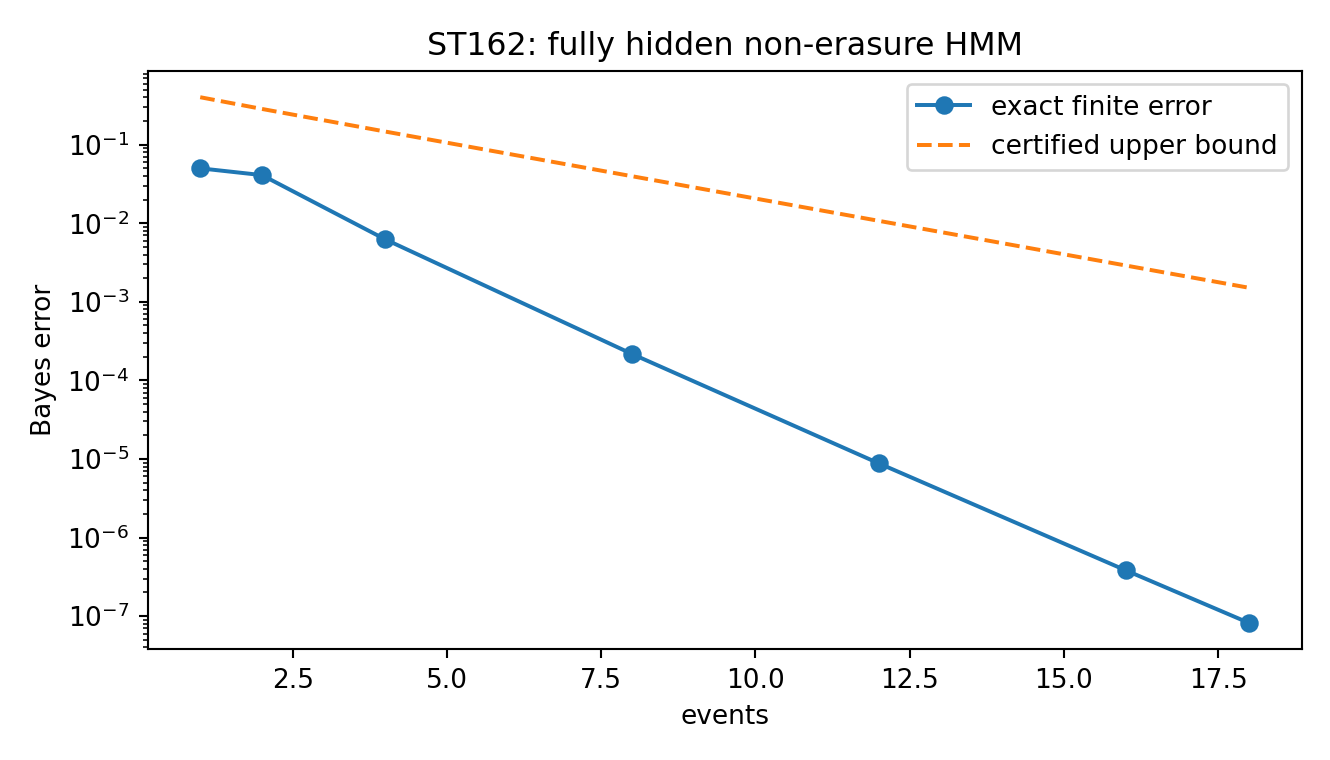
\includegraphics[width=.74\textwidth]{FIN_ST154_ST165_Figures/st162_hidden_hmm.png}
\caption{ST162. Corrected exact finite-count error and the conservative pair-path upper bound.}
\end{figure}

The theorem proves that temporal hiddenness does not automatically destroy exponential discrimination. It does not give the exact asymptotic Chernoff rate, and its strongly separated emissions are supplied.

\section{ST163: finite-time and site-local bath resources}

At supplied $\beta=0.8$, let $\gamma=e^{-\beta A}/\operatorname{Tr}(e^{-\beta A})$ and $\gamma_{\min}=0.0394461031$. The Gibbs replacement channel differs from the identity channel by at least
\[
D_0=2(1-\gamma_{\min})=1.9211077937
\]
in diamond norm, as witnessed by the least-populated energy eigenstate.

If a dilation generator has norm at most $g$ and $gt\le\pi$, then
\[
\|\mathcal E_t-\operatorname{Id}\|_\diamond\le4\sin(gt/2).
\]
Therefore any $\epsilon$-approximation to Gibbs replacement satisfies
\begin{equation}
t\ge\frac2g\arcsin\left(\frac{D_0-\epsilon}{4}\right).
\label{eq:speed}
\end{equation}
For exact reset, $gt\ge1.0019408674$. The isospectral two-qudit interaction $H_{\rm int}=g\,\mathrm{SWAP}$ is site-local, commutes with total equal Hamiltonian, and completes exact SWAP at $gt=\pi/2$.

\begin{figure}[H]\centering
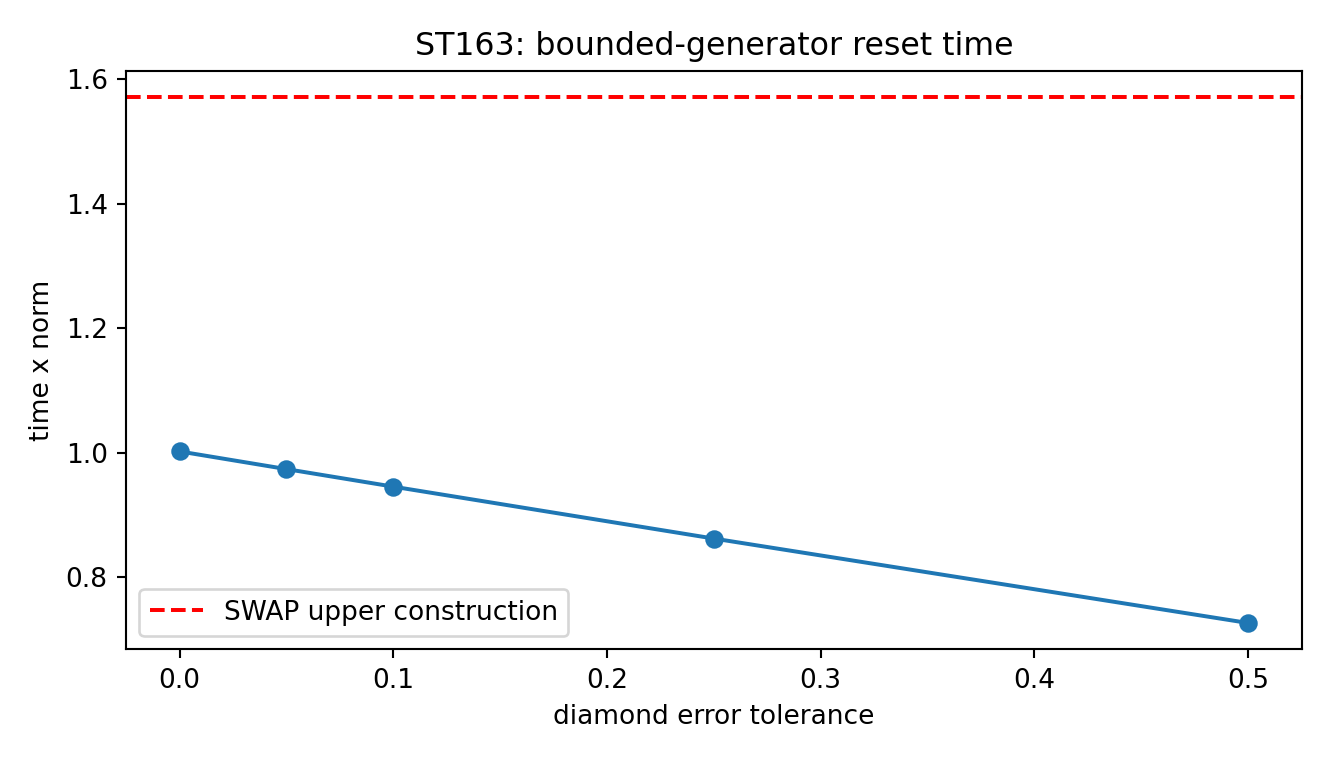
\includegraphics[width=.73\textwidth]{FIN_ST154_ST165_Figures/st163_bath_speed.png}
\caption{ST163. General speed lower bound and the explicit SWAP upper construction.}
\end{figure}

Together with ST152, exact reset requires bath dimension at least twelve and nonzero time under bounded generators. Microscopic qubit locality, Lieb--Robinson geometry, control restrictions, physical energy scale, and apparatus remain open.

\section{ST164: geometry of the minimax optimizer set}

The real minimax set is
\[
\mathcal S=\left\{H\succeq0:\ H_{ii}=\frac1{12},\ H_{ij}\ge0\ (i\ne j)\right\}.
\]
It has affine dimension $\binom{12}{2}=66$, because positive-definite matrices with strictly positive off-diagonal entries exist in its relative interior.

Write $H=VV^T$, with row vectors $v_i\in\mathbb R^r$, and let $Z$ be the zero off-diagonal positions.

\begin{theorem}[Complete linear extremality criterion]
$H$ is extreme in $\mathcal S$ if and only if the only $R\in\operatorname{Sym}_r$ satisfying
\[
v_i^TRv_i=0\quad\forall i,
\qquad v_i^TRv_j=0\quad\forall(i,j)\in Z
\]
is $R=0$.
\end{theorem}

Every set partition $\pi$ of the twelve labels gives a block-correlation extreme point: entries are $1/12$ within blocks and zero between blocks. Hence the set has at least
\[
B_{12}=4{,}213{,}597
\]
distinct extreme points. The certified examples range from rank twelve ($I/12$) to rank one ($J/12$).

\begin{figure}[H]\centering
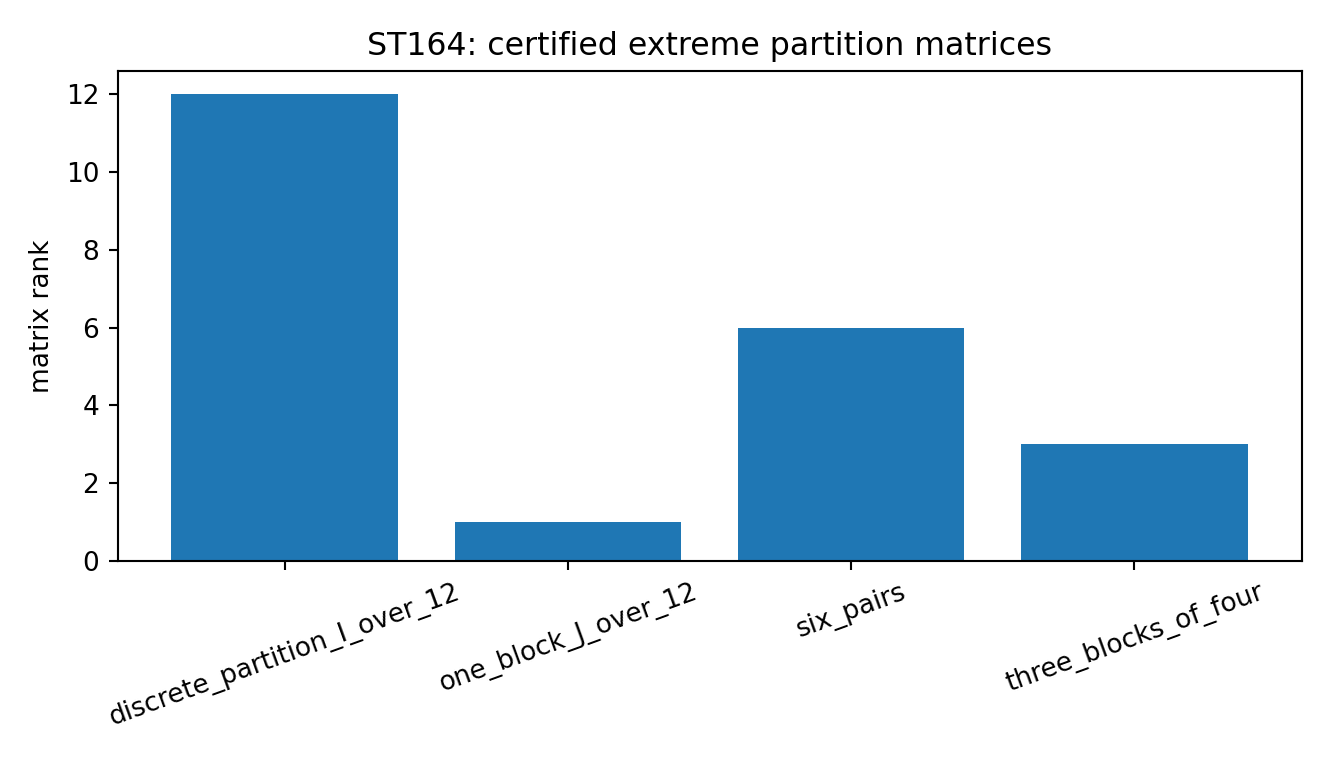
\includegraphics[width=.76\textwidth]{FIN_ST154_ST165_Figures/st164_extreme_partitions.png}
\caption{ST164. Ranks of representative certified partition extreme points.}
\end{figure}

The criterion is complete, but the full extreme-point list beyond the partition family has not been enumerated.

\section{ST165: the operational FIN completion tuple}

The studies now support the following typed completion:
\begin{equation}
\begin{aligned}
\mathcal O_{\rm FIN}=(&A_{\rm strict},\mathrm{ALG},\mathrm{GAUGE},\mathrm{PREP},
\mathrm{DYN},\mathrm{CLOCK},\mathrm{INST},\\
&\mathrm{ENV},\mathrm{APP},\mathrm{SELECT},\mathrm{UNITS},\mathrm{RECORD}).
\end{aligned}
\label{eq:tuple}
\end{equation}

The eleven added atoms respectively provide observable/composition typing, carrier equivalence, preparations, channel dynamics, calibrated duration, instruments, environment/bath, apparatus calibration, realized branch, dimensional scale, and an externally frozen event history.

Each atom has an explicit independence witness while $A$ is unchanged: spectral versus vertex algebras; trivial versus commutant gauge; uniform versus vertex preparation; unitary versus heat dynamics; $t$ versus $2t$ clock calibration; spectral versus vertex instruments; closed versus Gibbs-bath evolution; detector relabelings; any two ST147 branches; scale $u$ versus $cu$; and empty versus timestamped records.

\begin{proposition}[Relative axiom deletion]
Relative to the eleven declared operational obligations, deleting any atom from~\eqref{eq:tuple} removes the obligation assigned to it, while strict $A$ admits inequivalent choices of that atom. No atom is therefore determined from $A$ by type alone.
\end{proposition}

This is signature-minimal relative to the stated obligations, not an absolute theorem that no alternative formalism can combine several atoms. In particular, source, provider, registrar, analyst, and independent custody cannot be generated by local code merely by adding a field to the tuple.

\section{Information independent of a carrier: current answer}

The proposition that information is independent of a particular medium becomes mathematically meaningful only after defining:
\[
\text{encoding}\quad E_1,E_2,qquad
\text{instruments}\quad\mathsf I_1,\mathsf I_2,qquad
\text{comparison map}\quad T,
\]
and an operational invariant $\mathcal J$ satisfying
\[
\mathcal J(E_1,\mathsf I_1)=\mathcal J(E_2,\mathsf I_2).
\]
ST154 shows that different carrier interactions produce different observable algebras. ST160 supplies path-independent transport under a declared refinement functor. ST161 shows when instruments reconstruct the same factor structure. ST165 records gauge/equivalence as an indispensable atom. Together these results support a precise future program of representation-independent information, but do not prove that information exists without any physical realization.

Likewise, the existence of pinching, quotient, coarse-graining, and thermal maps is compatible with a projection interpretation of observed physics. It does not prove that the universe is a projection of FIN. A projection theorem would still need strict-derived encoding, selector, scale, instrument, and observation maps.

\section{Recommended programs ST166--ST177}

\begin{longtable}{@{}p{0.07\textwidth}p{0.10\textwidth}p{0.73\textwidth}@{}}
\toprule ID & Priority & Bounded research target\\\midrule\endfirsthead
\toprule ID & Priority & Bounded research target\\\midrule\endhead
ST166 & 1 & Define and falsify a carrier-change operational invariant under explicit encoding, decoding, and instrument functors.\\
ST167 & 2 & Derive an environment interaction observable from strict data, or prove a strict-source obstruction.\\
ST168 & 3 & Interval-cover a compact symmetry-reduced fold domain with both inclusion and exclusion boxes.\\
ST169 & 4 & Solve nonorthogonal coherent-unitary recovery using primal--dual SDP certificates.\\
ST170 & 5 & Derive selector cost from a declared Lindbladian or information-geometric control law.\\
ST171 & 6 & Search for a strict source of the local degree-twelve coupling $g$, or prove a coefficient no-go.\\
ST172 & 7 & Extend adaptive nuisance continuation until a certified geometric boundary or a declared resource stop.\\
ST173 & 8 & Lift refinement cohomology to noisy approximate functors and multiscale/fractal compression.\\
ST174 & 9 & Certify atomic-net reconstruction under finite tomography noise.\\
ST175 & 10 & Compute a sharper hidden-HMM Chernoff rate using interval Lyapunov or transfer-operator methods.\\
ST176 & 11 & Derive reset bounds for microscopic $k$-local bath encodings and Lieb--Robinson geometry.\\
ST177 & 12 & Implement the ST165 operational tuple as an executable validator with frozen record and axiom-deletion tests.\\
\bottomrule
\end{longtable}

ST166 has the highest conceptual value because it turns ``information independent of medium'' into a falsifiable equivalence problem. ST167 and ST171 are the most direct strict-source tests. ST168 is the strongest local proof opportunity.

\section{Reproducibility and audit trail}

The executable source is \texttt{fin\_st154\_st165\_research.py}. It writes the master JSON, CSV outcome table, nine specialized certificate/result packets, and nine figures. The deterministic seed is \texttt{20260824}. The recorded environment is Python 3.12.3, NumPy 1.26.4, and SciPy 1.17.1.

The test suite \texttt{test\_fin\_st154\_st165.py} contains 34 checks. It detected the first-event enumeration defect in the initial ST162 implementation; that implementation was corrected and every result regenerated. Live checks cover commutants, fold shells, stochastic readout, recovery, action formulas, exact anisotropy coefficients, the 64-cell cover, refinement fibers, instrument algebras, normalized HMM likelihoods, Chernoff bounds, reset speed, Bell numbers, extremality ranks, and operational deletion witnesses.

File integrity is recorded in \texttt{FIN\_ST154\_ST165\_SHA256SUMS.txt}. No external laboratory data or external audit is used.

\section{Final verdict}

\resultbox{\textbf{Deepest surviving interpretation.} FIN remains a finite spectral-information core whose possible physical realization requires a typed operational completion. This batch shows exactly how two missing structures could arise: an observable algebra from environmental interaction, and twelvefold anisotropy from the first lattice-allowed local nonlinearity. In both cases the remaining coupling/source is independent of strict functional calculus. The theory has therefore gained sharper mechanisms and sharper obstructions, not a hidden zero-axiom transition to physics.}

No strict environment coupling, fine algebra, QW-2191 discharge, strict anisotropy coefficient, dimensional unit, calibrated physical clock, apparatus, independent record, laboratory result, legacy-to-strict completion, legacy physical-role transfer, Standard Model, gravity, total physical Lagrangian, physical projection theorem, or Theory-of-Everything closure is claimed.

\end{document}
